\documentclass[9pt]{article}
\usepackage{amsmath,amsfonts,amssymb, times}
\usepackage{graphicx,color,tikz,pgfplots}
\usepackage[paperwidth=9cm,paperheight=5.5cm,lmargin=0in,rmargin=0in,tmargin=4pt,bmargin=0.in]{geometry}
\usepackage{bm}
\usetikzlibrary{arrows,shadings,shapes.arrows,decorations.pathreplacing,calc}
\usepgfplotslibrary{fillbetween}


\pagestyle{empty}
\pgfplotsset{compat=newest}
\definecolor{applered}{RGB}{255,8,0}
\definecolor{azure}{RGB}{0,127,255}
\definecolor{violet}{RGB}{159,0,255}

\pgfdeclareverticalshading{rainbow}{100bp}
{color(0bp)=(applered); color(25bp)=(red); color(40bp)=(yellow);
  color(47bp)=(green); color(51bp)=(cyan); color(60bp)=(blue);
  color(65bp)=(violet); color(100bp)=(violet)} 
                          
\newlength{\h}
\newlength{\rad}
\setlength{\h}{0.5cm}
\setlength{\rad}{1.5pt}

\begin{document}
\centering
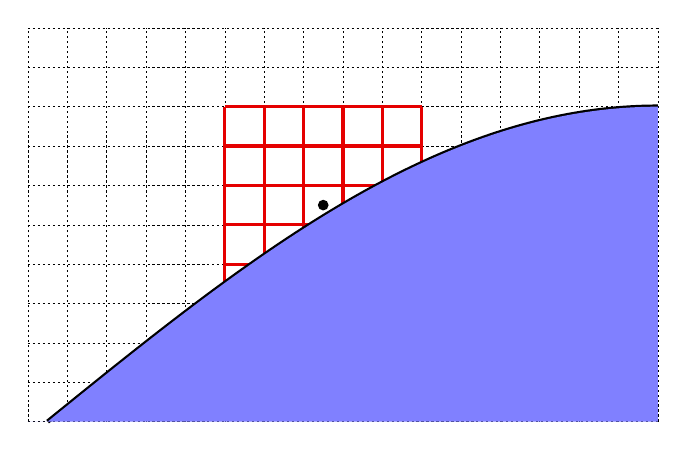
\begin{tikzpicture}[
    gridstyle/.style={thick,black, densely dotted},
    nodeCenterStyle/.style={thick,black,fill},
    nodeFaceStyle/.style={thick,black},
    VoFStyle/.style={font=\small,anchor = north west},
    surfaceStyle/.style={ultra thick,black},
    volumeStyle/.style={thick,densely dashed,black},
    surfaceFill/.style={},
    braceStyle/.style={thick,decorate,decoration={brace,amplitude=4pt,raise=2pt}},
    alphaStyle/.style={font=\small,anchor=east,xshift=-4pt},
    hTopStyle/.style={font=\small,anchor=east,yshift=4pt},
    hLeftStyle/.style={font=\small,anchor=east,xshift=-4pt},
    betaStyle/.style={font=\small,anchor=west,xshift=4pt},
    EBStyle/.style={font=\small,anchor=south,yshift=4pt},
    kappaStyle/.style={font=\small,anchor=center},
    normalStyle/.style={font=\small,->,thick,black},
    gradientStyle/.style={font=\small,->,thick,black},
    surfaceCharge/.style={font=\small,yshift=2pt},
    phiStyle/.style={font=\small,anchor=south},
  ]

  %% Grids and nodes
  \draw[step=\h,gridstyle, very thin] (0,0) grid (16\h,10\h);

  \path[name path=baseline] (0,0) -- (16\h,0\h);

  \draw[nodeCenterStyle] (7.5\h, 5.5\h) circle(\rad);

  \draw[step=\h, draw=red!90!black, very thick, fill=red!70!white] (5\h,3\h) grid (10\h,8\h);
  \draw[surfaceStyle,name path=surface] (0.5\h,0) sin (16\h,8\h);
  \tikzfillbetween[of=surface and baseline,on layer=,every segment/.style={surfaceFill}] {blue!50!white};


  
\end{tikzpicture}
\end{document}
